% First page
\thispagestyle{plain}
  \begin{center}
    \includegraphics[scale=1]{"hua.png"}\\
    \vspace{1cm}
    {\huge ΧΑΡΟΚΟΠΕΙΟ ΠΑΝΕΠΙΣΤΗΜΙΟ}\\
        \vspace{1cm}
    {\Large ΣΧΟΛΗ Ψηφιακής Τεχνολογίας}\\
    {\Large ΤΜΗΜΑ Πληροφορικής και Τηλεματικής}\\
        \vspace{5cm}
    {\large \textit{Ανάπτυξη εφαρμογής επεξεργασίας δυαδικών αρχείων}}\\
       \vspace{1cm} 
  \textit{Πτυχιακή εργασία}\\
    {\large Κατσιφώλης Βασίλης}\\
    
    \vspace{1cm}
    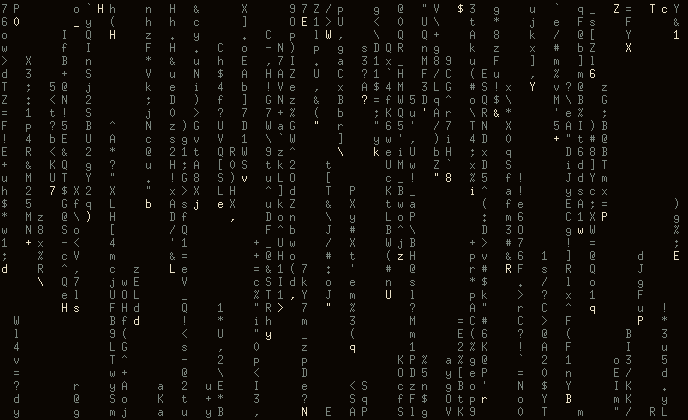
\includegraphics[scale=0.5]{"static/cover.png"}\\
    \vspace{3cm}
    Αθήνα, 2021\\

  \end{center}
\pagebreak

% Second page
  \begin{center}
    {\huge ΧΑΡΟΚΟΠΕΙΟ ΠΑΝΕΠΙΣΤΗΜΙΟ}\\
    \vspace{4cm}
    ΣΧΟΛΗ Ψηφιακής Τεχνολογίας \\
    ΤΜΗΜΑ Πληροφορικής και Τηλεματικής\\
    \vspace{4cm}
    \textbf{Τριμελής Εξεταστική Επιτροπή}\\
    
 	Επιβλέπων\\
    Κωνσταντίνος Τσερπές\\
    Επίκουρος Καθηγητής, Πληροφορικής και Τηλεματικής, Χαροκόπειο Πανεπιστήμιο\\[1\baselineskip]
    Μέλη\\
    Ανάργυρος Τσαδήμας\\
    Ε.ΔΙ.Π, Τμήμα Πληροφορικής και Τηλεματικής, Χαροκόπειο Πανεπιστήμιο\\[1\baselineskip]
    Γεώργιος Κουσιουρής\\
    Επίκουρος Καθηγητής, Πληροφορικής και Τηλεματικής, Χαροκόπειο Πανεπιστημιό\\
   
  \end{center}
\pagebreak

% Third (agreement) page
Ο Κατσιφώλης Βασίλης δηλώνω υπεύθυνα ότι:

\begin{enumerate}
\item Είμαι ο κάτοχος των πνευματικών δικαιωμάτων της πρωτότυπης αυτής εργασίας και από όσο γνωρίζω η εργασία μου δε συκοφαντεί πρόσωπα, ούτε προσβάλει τα πνευματικά δικαιώματα τρίτων.
\item Αποδέχομαι ότι η ΒΚΠ μπορεί, χωρίς να αλλάξει το περιεχόμενο της εργασίας μου, να τη διαθέσει σε ηλεκτρονική μορφή μέσα από τη ψηφιακή Βιβλιοθήκη της, να την αντιγράψει σε οποιοδήποτε μέσο ή/και σε οποιοδήποτε μορφότυπο καθώς και να κρατά περισσότερα από ένα αντίγραφα για λόγους συντήρησης και ασφάλειας.
\end{enumerate}

% Eyxaristies
\pagebreak
\section*{Ευχαριστίες}
Η παρούσα πτυχιακή εργασία πραγματοποιήθηκε στο Χαροκόπειο Πανεπιστήμιο Αθηνών, στο τμήμα Πληροφορικής και Τηλεματικής κατά το έτος 2021.

Στα πλαίσια της εκπόνηση της πτυχιακής μου εργασίας θα ήθελα να ευχαριστήσω τον κ. Τσερπέ Κωνσταντίνο για την πολύτιμη βοήθεια του και την υπομονή που έδειξε καθόλη τη διάρκεια ολοκλήρωσή της.

Θα ήθελα να ευχαριστήσω τα αγαπημένα μου πρόσωπα, του γονείς μου, τον αδερφό μου και τους φίλους μου οι οποίοι ο καθένας με τον δικό του ανεκτίμητο τρόπο είτε υλικό είτε πνευματικό, κατάφεραν να με βοηθήσουν να φτάσω σε αυτό το σημείο και συνεχίζουν να το κάνουν, μέχρι και σήμερα.


\pagebreak
